\section{Introduction}

\emph{If you know your enemies and know yourself, you will not be imperiled in a hundred battles~\cite{WikiquoteSunTzu}.} This is the quote by Sun Tzu (c. 6th century BCE), who was a Chinese general, military strategist, and author of the book The Art of War, an immensely influential ancient Chinese book on military strategy. This quote is the one of the principle of empirical software engineering. To know your \emph{enemies} (i.e., bugs) and \emph{yourself} (i.e., software systems) and win \emph{battles} (i.e., leading a project to success conclusion), one needs to investigate a large amount of research on Software Quality Assurance (SQA). SQA can be broadly defined as the set of activities that ensure software meets a specific quality level~\cite{Fenton1999TSE}.

%\para{we explain why software is important. Everybody use software as not only infrastructure but also daily wants (e.g., mobile apps). We also show how much money are lost by bugs. } \todo{Need to find some papers that say how much money are lost by bugs in the domain of infra and mobile apps.}

As software systems continue to play an increasingly important role in our lives, their complexity continues to increase; making SQA efforts very difficult. At the same time, the importance of SQA efforts is of paramount importance, as shown by the US National Institute of Standards and Technology (NIST) study, which estimated that software faults and failures cost the US economy \$59.5 billion a year~\cite{NIST}. Therefore, to ensure high software quality, software defect prediction models, which describe the relationship between various software metrics (e.g., SLOC and McCabe's Cyclomatic complexity) and software defects, have been proposed~\cite{Zimmermann2007,Moser2008ICSE}. Traditionally, the software defect prediction models are used in two ways: (1) to predict where defects might appear in the future and allocate SQA resources to defect-prone artifacts (e.g., subsystems and files)~\cite{Munson1992} and (2) to understand the effect of factors on the likelihood of finding a defect and derive practical guidelines for future software development projects~\cite{Cataldo2009TSE,McIntosh2014MSR}.

%We still eagerly focus on SQA studies, software systems are becoming complexity and being used in everything from mobile devices to artificial satellites. The increasing importance and complexity make the quality of software systems critical and rise the cost of SQA activities. For example, the  Since a company has only limited resources (e.g., developers and cost) for SQA activities, these activities have to be performed as efficiently as possible.

% http://blog.typemock.com/2012/05/what-is-the-cost-of-avoiding-unit-testing-and-the-cost-of-software-bugs.html

%\para{To know bugs, many studies about software quality assurance (SQA) are conducted, especially using empirical approaches.} We introduce one of oldest empirical papers and a couple of papers? Bug prediction (defect prediction. We define what bug prediction is.) \yasu{I would like to explain not only ``prediction'', but also ``understanding'' in our context}.

%One line of work that have received a lot of attention in recent years is defect prediction models, which describe the relationship between factors (e.g., SLOC and McCabe's Cyclomatic complexity) as predictor variables and a status (e.g., defect-prone or not after releases) as a response variable~\cite{Ohlsson1996TSE,Zimmermann2007,Moser2008ICSE}. The models can be used as (1) to predict where defects might appear in the future and allocate SQA resources to defect-prone artifacts (e.g., subsystems and files)~\cite{Munson1992, } and (2) to understand the effect of factors on the likelihood of finding a defect and derive practical guidelines for future software development projects~\cite{Cataldo2009TSE,McIntosh2014MSR}.

Due to its importance, defect prediction work has been at the focus of researchers for over 40 years. As Fenton and Neil~\cite{Fenton2000ICSE} explained, Akiyama~\cite{Akiyama1971IFIP} first attempted to build defect prediction models using size-based metrics and regression modelling techniques in 1971. Since then, there have been many studies and many accomplishments in software defect prediction. At the same time, there remain many challenges that face software defect prediction. Hence, we find that it is a perfect time to write a Future of Software Engineering (FoSM) paper on the topic of software defect prediction.

The paper is written from a budding university researchers' point of view and aims to accomplish \todo{three} things. First, we provide a brief overview of software defect prediction and its various components. Second, we revisit the challenges of software prediction models as they were seen in the year 2000, in order to reflect on our accomplishments since then. We also highlight our accomplishments and recent trends, as well as, discuss the game changers that had a significant impact on software defect prediction. Third, we highlight some key challenges that lie ahead in the near (and not so near) future in order to us as a research community to tackle these future challenges.

%his areaAfter the first publication, there are many studies on defect prediction models~\cite{Ohlsson1996TSE,Zimmermann2007,Moser2008ICSE}. In addition, thanks to the rich and readily available software repositories from modern software development environments, the defect prediction model filed is accelerating research speed and uncovering useful information about software projects.

%However, we still have many challenges in the field of software defect prediction. In this paper, we would like to highlight some key challenges for future (from budding university researchers' point of view). 

\begin{figure*}
  \centering
  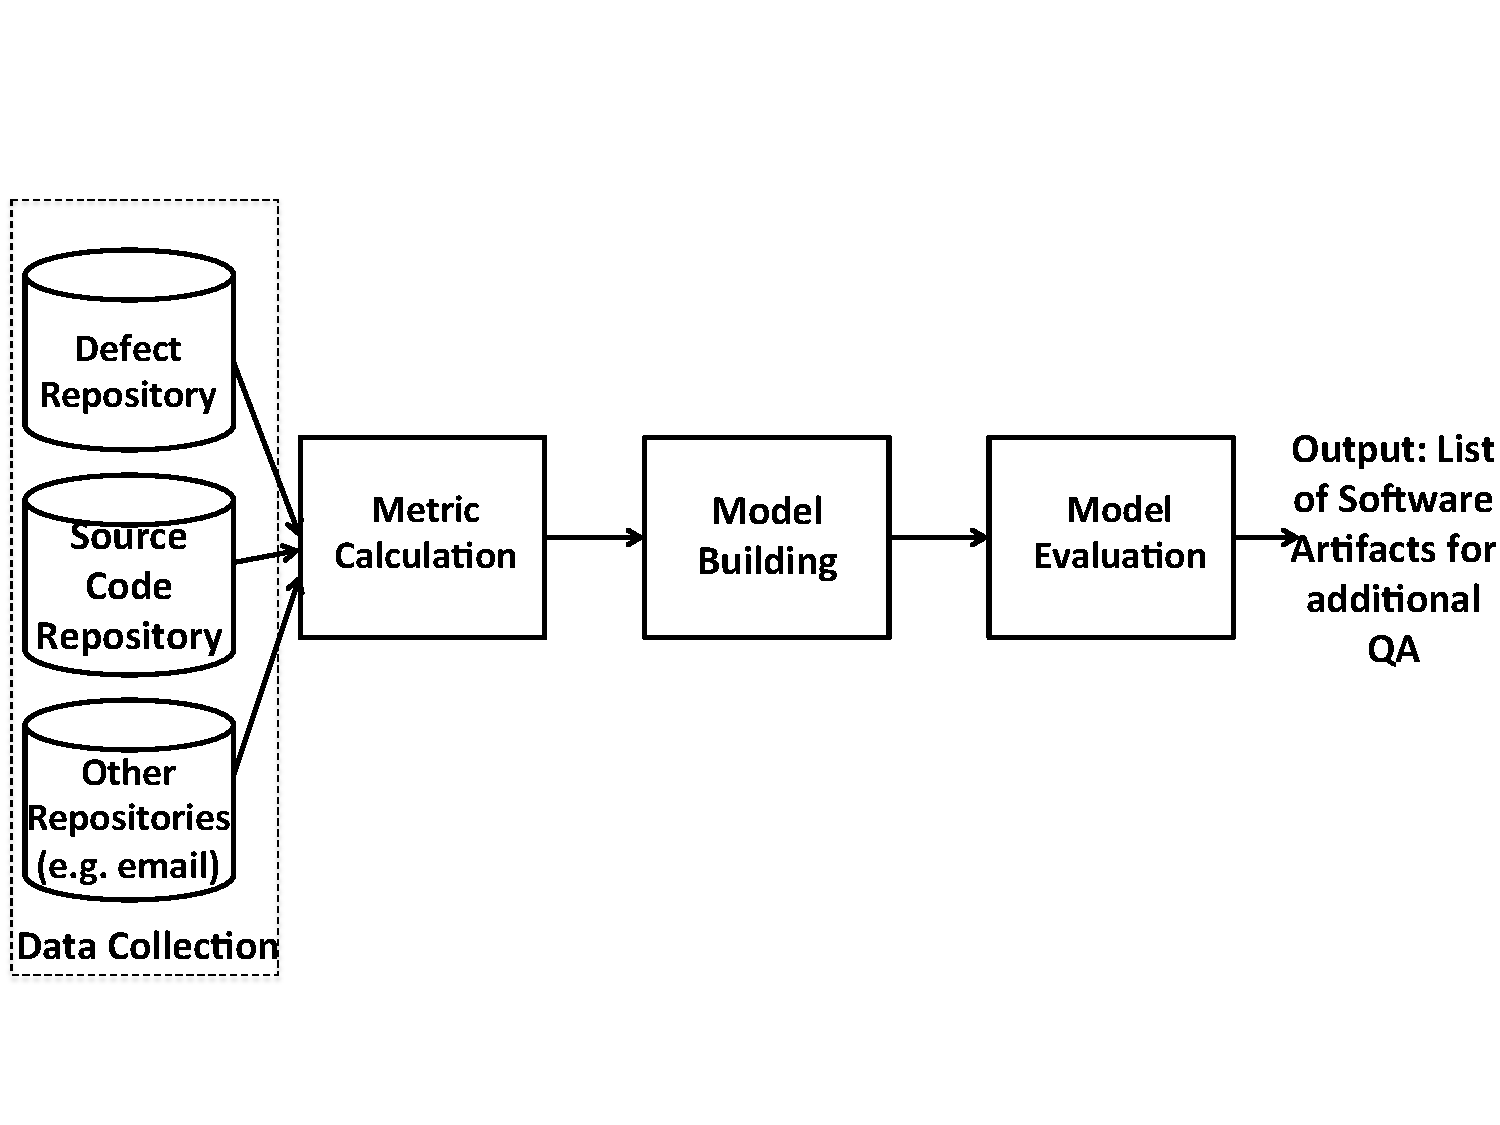
\includegraphics[trim=0 60 0 80, scale=0.5,clip] {figures/overview}
  \caption{Overview of Software Defect Prediction (SDP)~\cite{Shihab2012PhD} \label{fig:overview}}
\end{figure*}

\smallsection{Target Readers} We hope that all researchers and practitioners, especially masters students, PhD students and young researchers, read this paper in order to gain an understanding of whole pictures of defect prediction studies and some key challenges for future, then share their opinion and discuss the future of software quality assurance with us.

\smallsection{Paper Organization} To purse the goal of this paper, the paper is organized as follows. 
Section \ref{background} explains the overview of defect prediction models.
Section \ref{past} revisits what challenges were in Year 2000.
%Section \ref{trends} assesses what state the research trend is in.
%Section \ref{game_changers} presents game changers, which dramatically changed perspective and direction of the studies in the field of defect prediction.
Section \ref{trends} assesses what state the research trend is in and presents some of game changers, which dramatically changed perspective and direction of the studies in the field of defect prediction.
Section \ref{challenges} highlights some key challenges for future.
Section \ref{conclusion} draws conclusions.
